% ============================================================
% Section 5.2: Virtual Keyboard Performance Results
% ============================================================
\section{Virtual Keyboard Performance Results}
\label{sec:virtual_keyboard_performance}

To evaluate the system's ability to provide independent communication for motor-impaired patients, the Graphical User Interface (GUI) programmed in MATLAB was tested. The virtual keyboard was designed specifically for patients with quadriplegia, Locked-in Syndrome (LIS), and muscular dystrophy, using an automatic scanning mechanism to minimize physical and mental effort.

Figure \ref{fig:virtual_keyboard_main_interface} shows the main layout of the virtual keyboard. The interface is divided into six circular sectors containing strategically arranged Arabic letters and commands. The system automatically scans through these sectors sequentially. When the user performs a voluntary blink that exceeds the programmed voltage threshold, the active sector is selected. The system then immediately switches to scanning the individual letters within that sector for selection with a second blink.

\begin{figure}[H]
  \centering
  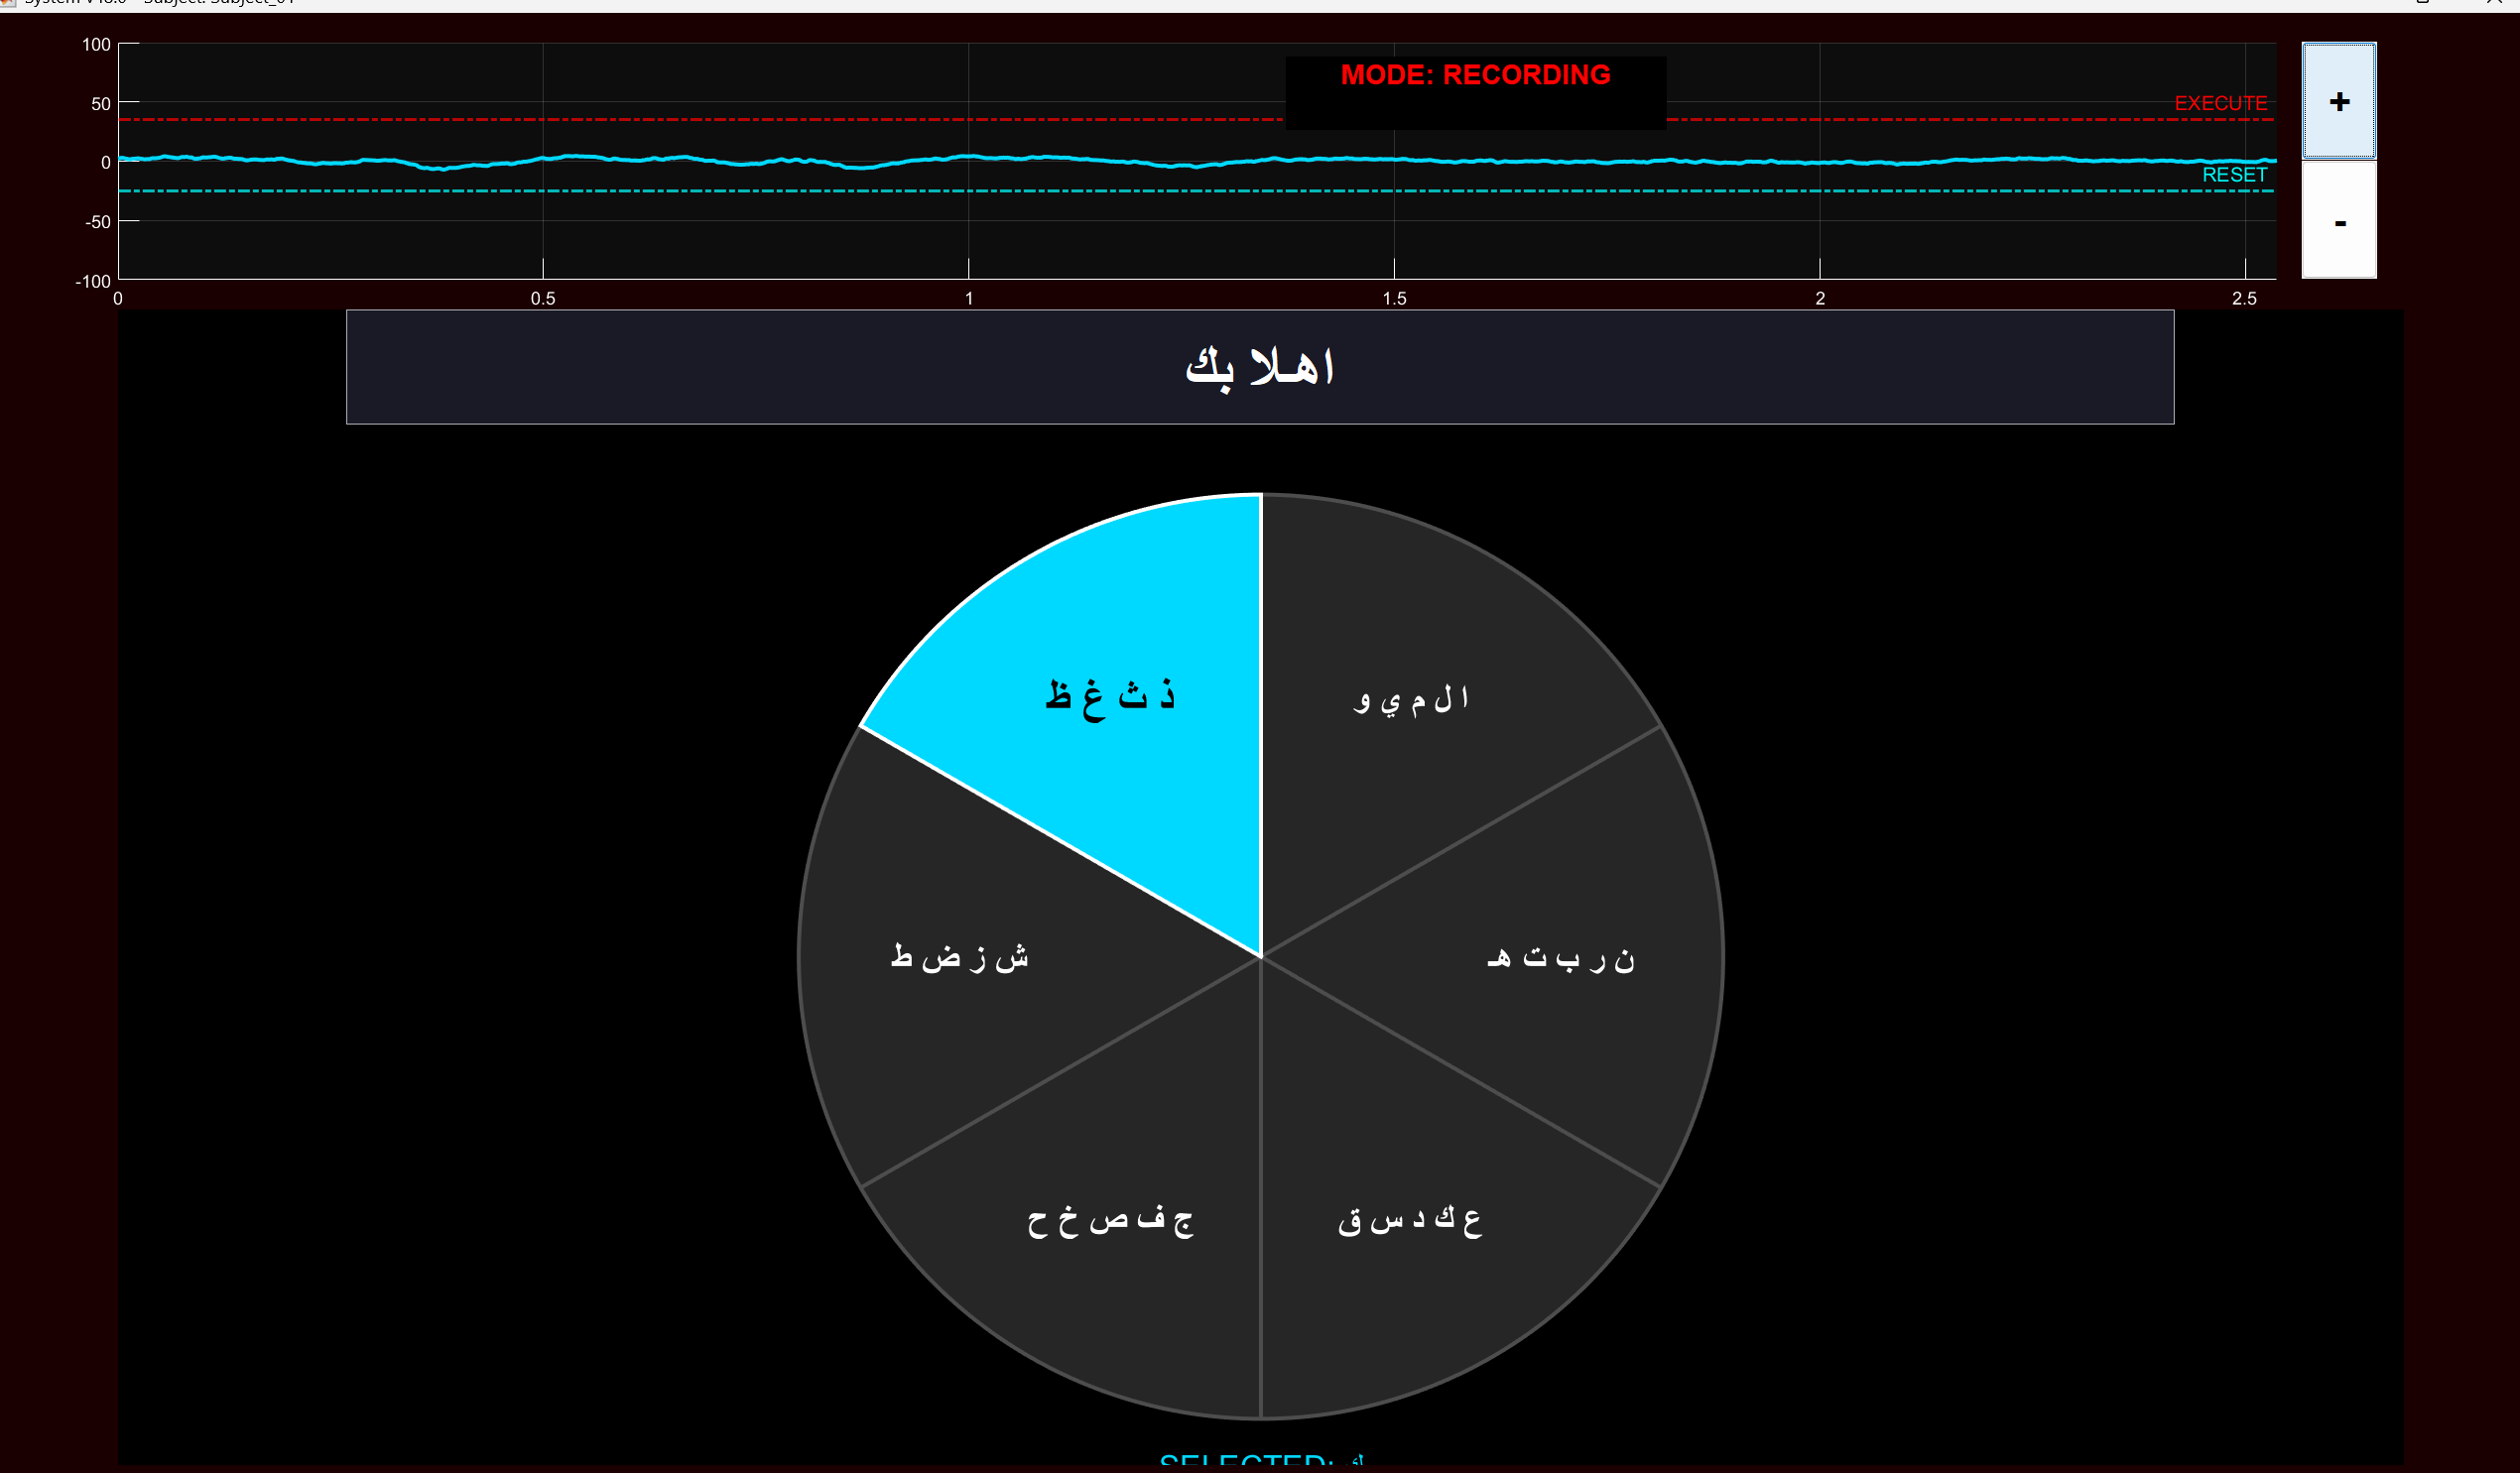
\includegraphics[width=0.85\textwidth]{03_Figures/Ch5/virtual_keyboard_main_interface.png}
  \caption{Virtual keyboard main interface.}
  \label{fig:virtual_keyboard_main_interface}
\end{figure}

Figure \ref{fig:character_selection_inside_sector} shows the sub-level scanning inside a selected sector. The individual letters and commands are scanned one by one. The top signal plot displays the real-time blink spike crossing the threshold line to confirm character selection, demonstrating a fast system response.

\begin{figure}[H]
  \centering
  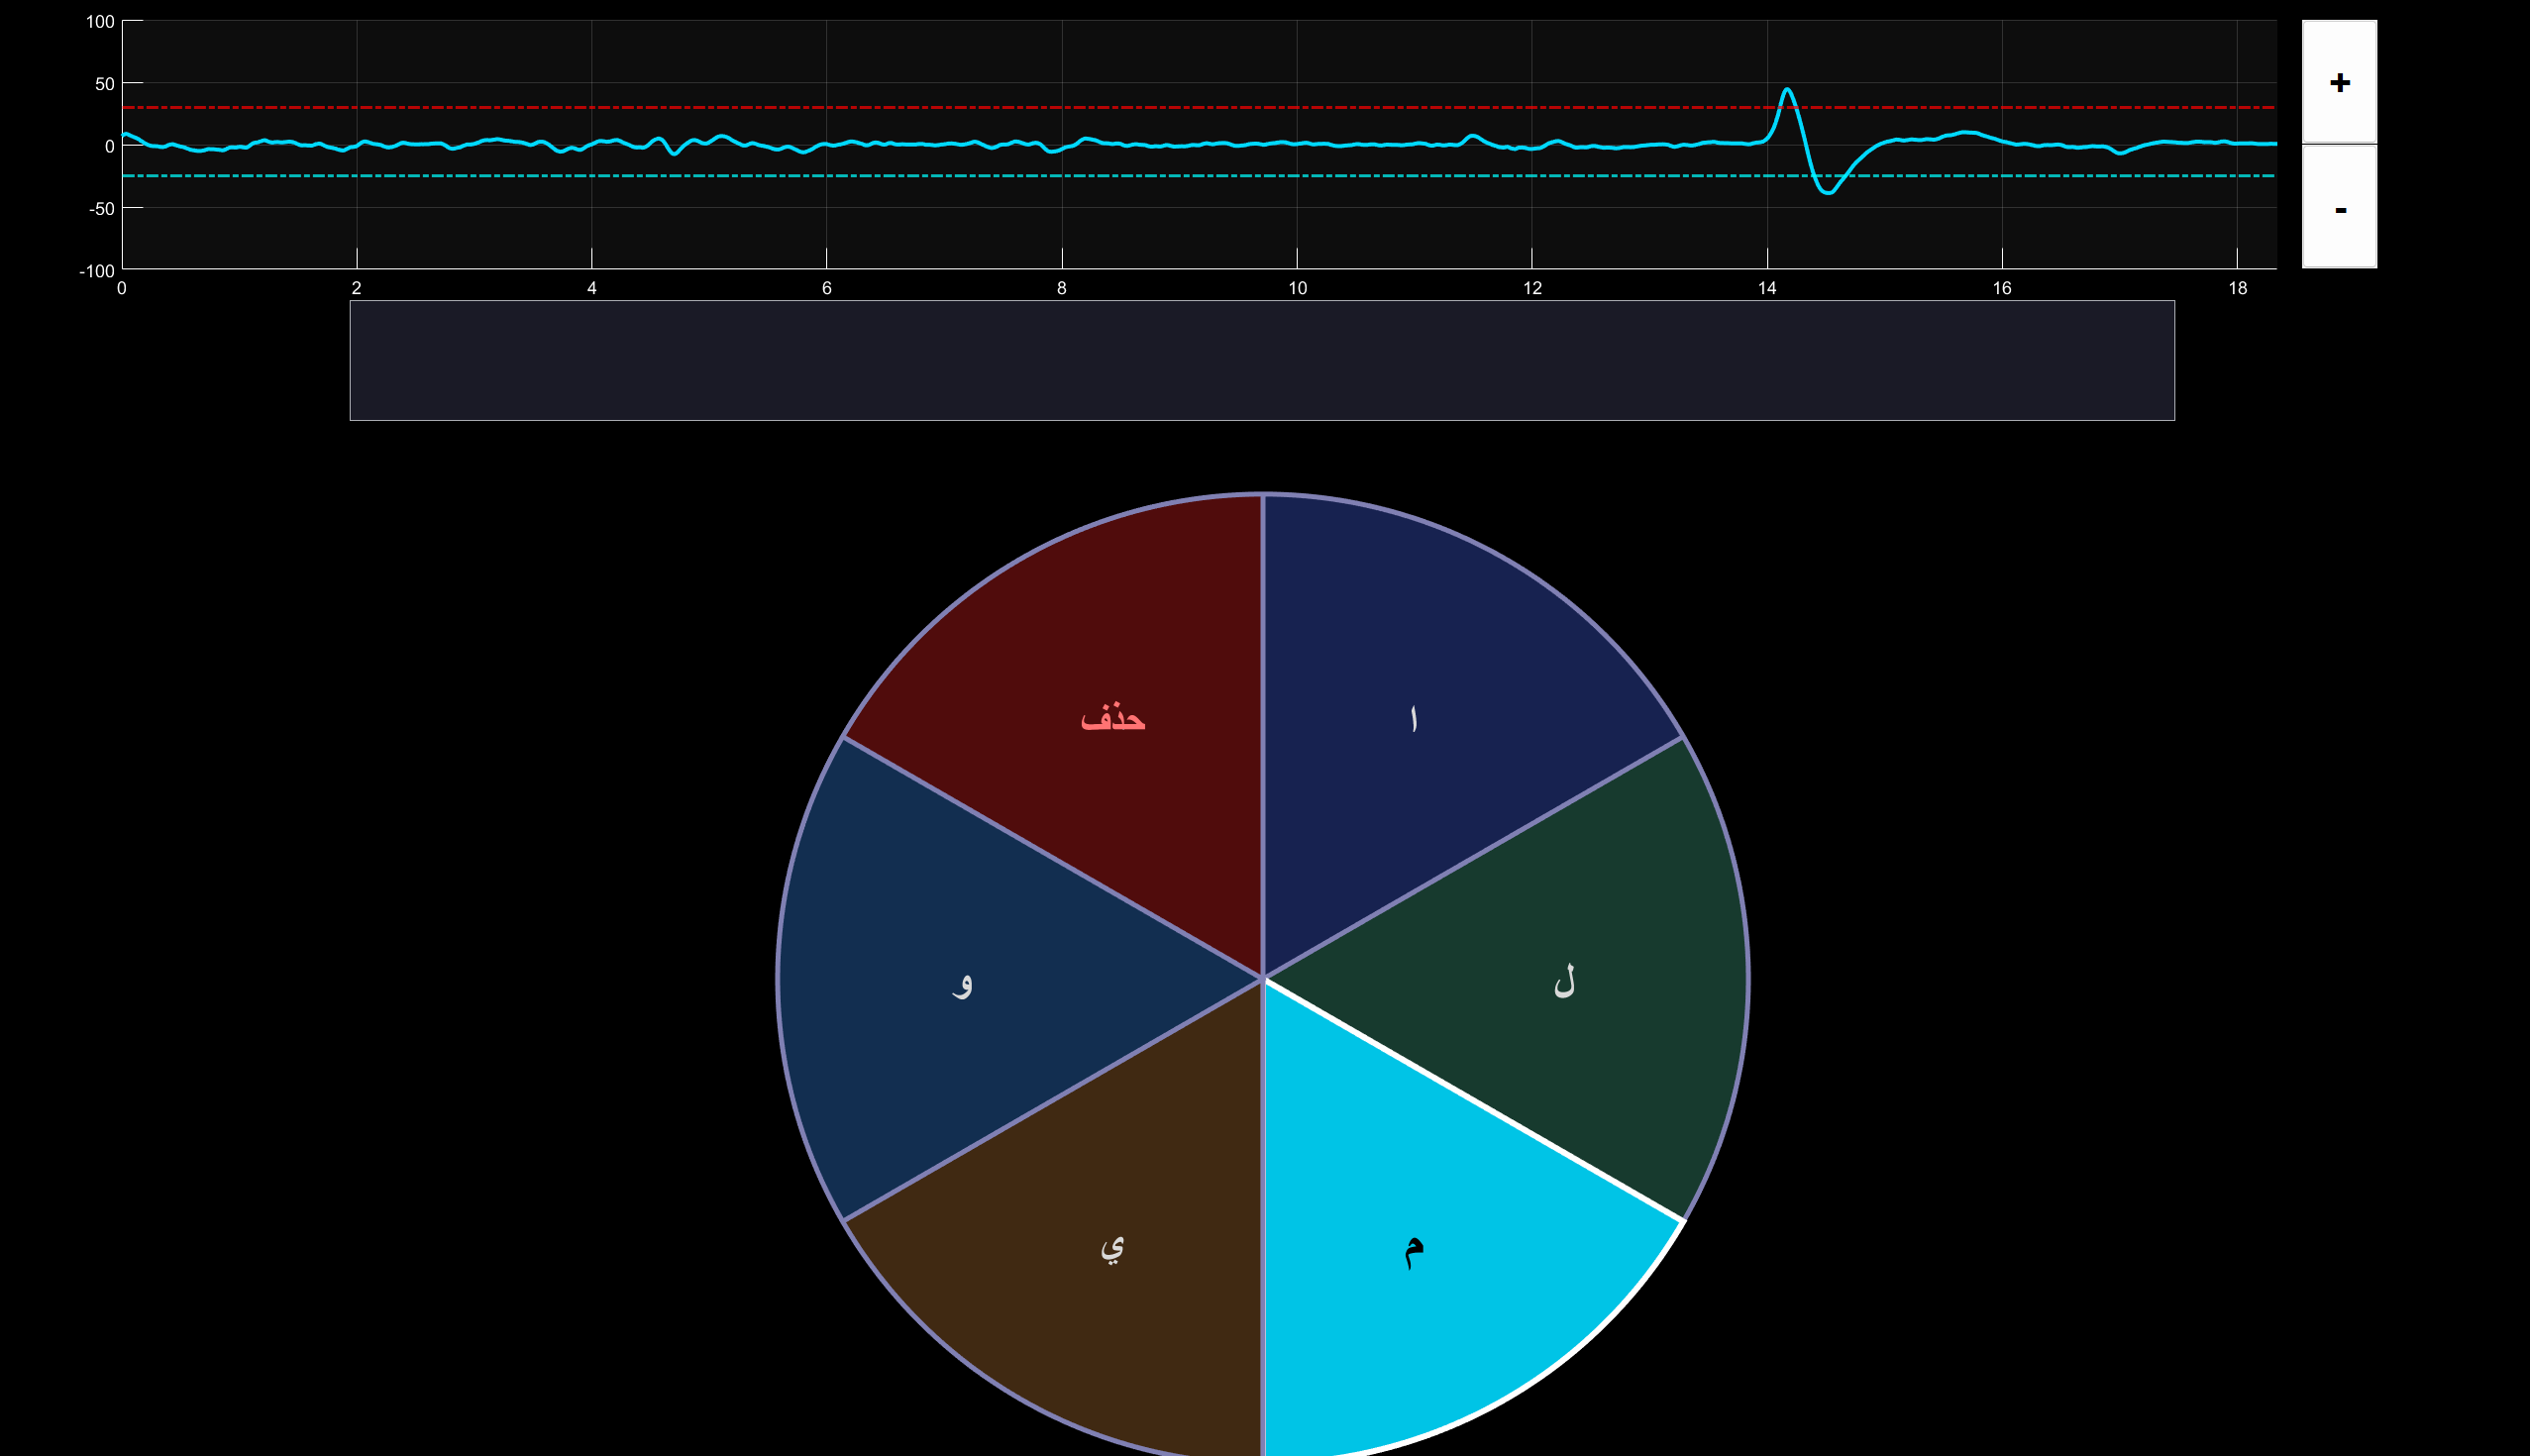
\includegraphics[width=0.85\textwidth]{03_Figures/Ch5/character_selection_inside_sector.png}
  \caption{Character selection inside a chosen sector.}
  \label{fig:character_selection_inside_sector}
\end{figure}

Experimental testing demonstrated high efficiency in translating eye blinks into written text at a comfortable scanning speed. A key advantage of this design is solving the ``Midas Touch'' problem---a common limitation in traditional camera-based eye-tracking systems where random gaze is incorrectly registered as an input. In this system, selection is triggered only by an intentional blink crossing the voltage threshold, significantly reducing false inputs and preventing eye strain.

Additionally, the system responded accurately to built-in editing features (such as space insertion, backspace, full text clearing, and group re-selection correction). This allows patients to independently compose sentences and express their needs without caregiver assistance.
